% 1988 年全国卷文科第 22 题：四棱锥 S-ABCD
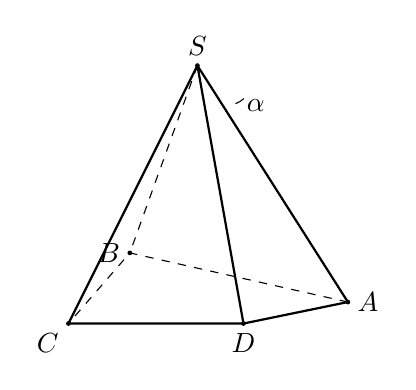
\begin{tikzpicture}[scale=0.78,>=stealth]
  \coordinate (S) at (2.1,4.2);
  \coordinate (B) at (1.0,1.15);
  \coordinate (A) at (4.55,0.35);
  \coordinate (D) at (2.85,0.0);
  \coordinate (C) at (0,0.0);
  \draw[thick] (S)--(C) (S)--(D) (S)--(A);
  \draw[dashed] (S)--(B);
  \draw[thick] (C)--(D)--(A);
  \draw[dashed] (A)--(B)--(C);
  \draw (2.72,3.58) arc (-70:-48:0.42);
  \node at (3.05,3.55) {$\alpha$};
  \fill (S) circle (1.1pt) node[above] {$S$};
  \fill (A) circle (1.1pt) node[right] {$A$};
  \fill (B) circle (1.1pt) node[left] {$B$};
  \fill (C) circle (1.1pt) node[below left] {$C$};
  \fill (D) circle (1.1pt) node[below] {$D$};
\end{tikzpicture}
